%================================================
% PACKAGES AND THEMES
%================================================
\documentclass[t,aspectratio=169,xcolor=dvipsnames]{beamer}

\usetheme{SimplePlusAIC}

\usepackage{graphicx}
\usepackage{booktabs}
\usepackage{svg}
\usepackage{tcolorbox}
\usepackage{tikz}
\usetikzlibrary{shapes.geometric, arrows, positioning, fit, calc}
\usepackage{makecell}

\newcommand*{\defeq}{\stackrel{\text{def}}{=}}
\usepackage{setspace}
\usepackage[T1]{fontenc}
\usepackage{helvet}
\usepackage{textgreek}
\usepackage{amsmath}
\usepackage{bm}
\usepackage{ragged2e}
\usepackage{xfrac}
\usepackage[loose]{units}
\usepackage{braket}
\usepackage{physics}
\usepackage{gensymb}
\usepackage{verbatim}
\usepackage{fancyvrb}

\usepackage[svgnames,table]{xcolor}
\arrayrulecolor{black}
\setlength{\arrayrulewidth}{0.20mm}
\renewcommand{\arraystretch}{1.35}

\newcommand{\tem}[1]{\textbf{\textcolor{red}{#1}}}

%================================================
% TITLE PAGE
%================================================
\title[Memory Management]{Manajemen Memori}
\subtitle{Week 6: Fragmentasi, Alokasi, \& Paging}
\author[lectura.id/course/os]{lectura.id/course/os}
\institute[ITERA]{Program Studi Teknik Informatika \\ Institut Teknologi Sumatera}
\date{\textcolor{nyublue}{2026}}

%================================================
% BEGIN DOCUMENT
%================================================
\begin{document}

\begin{frame}
    \titlepage
\end{frame}

\begin{frame}
    \frametitle{OUTLINE}
    \framesubtitle{Peta materi pertemuan ini}
    \small
    \begin{spacing}{1.15}
        \tableofcontents
    \end{spacing}
\end{frame}

\begin{frame}
    \frametitle{Capaian Pembelajaran}
    \framesubtitle{Tujuan setelah pertemuan selesai}
    \small
    \begin{enumerate}
        \item Memahami masalah utama dalam alokasi memori dinamis.
        \item Menganalisis algoritma alokasi First-Fit, Best-Fit, dan Worst-Fit.
        \item Membedakan fragmentasi eksternal dan fragmentasi internal.
        \item Memahami konsep dasar Paging sebagai solusi manajemen memori noncontiguous.
        \item Menjelaskan cara kerja translasi alamat logis ke fisik pada Paging.
    \end{enumerate}
    \begin{exampleblock}{Fokus Kelas Ini}
        Kita akan mempelajari bagaimana OS mengalokasikan ruang memori, mengelola sisa ruang kosong (fragmentasi), dan teknik perbaikan melalui \tem{Paging}.
    \end{exampleblock}
\end{frame}

\section{Algoritma Alokasi Memori}

\begin{frame}
    \frametitle{Masalah Alokasi Dinamis}
    \framesubtitle{Bagaimana menempatkan proses ke memori?}
    \small
    \begin{itemize}
        \item OS memelihara \tem{tabel memori} yang mencatat blok terpakai dan blok kosong (\textit{hole}).
        \item Awalnya, memori adalah satu \textit{hole} besar.
        \item Saat proses-proses mulai berjalan dan berhenti, memori akan berisi kumpulan \textit{holes} berukuran berbeda-beda yang tersebar.
    \end{itemize}
    \vspace{0.2cm}
    \begin{alertblock}{Tantangan Utama}
        Ketika proses baru datang meminta memori sebesar $N$, \tem{\textit{hole} mana} dari daftar \textit{free holes} yang harus dipilih OS?
    \end{alertblock}
\end{frame}

\begin{frame}
    \frametitle{Tiga Strategi Utama Alokasi}
    \framesubtitle{Cara OS memilih ruang kosong}
    \small
    \begin{table}[]
        \centering
        \begin{tabular}{p{0.20\textwidth}p{0.33\textwidth}p{0.37\textwidth}}
            \toprule
            \textbf{Strategi} & \textbf{Cara Kerja} & \textbf{Karakteristik} \\
            \midrule
            \tem{First-Fit} & Pilih \textit{hole} \textbf{pertama} yang muat. & Pencarian berhentik cepat. Meninggalkan \textit{hole} kecil di awal memori. \\
            \tem{Best-Fit} & Pilih \textit{hole} \textbf{terkecil} yang muat. & Scan seluruh daftar. Sisa \textit{hole} sangat kecil. Baik untuk menghemat ruang. \\
            \tem{Worst-Fit} & Pilih \textit{hole} \textbf{terbesar} yang muat. & Scan seluruh daftar. Menyisakan \textit{hole} besar. Praktiknya sering kurang performanya. \\
            \bottomrule
        \end{tabular}
    \end{table}
\end{frame}

\begin{frame}
    \frametitle{Ilustrasi Strategi Alokasi}
    \framesubtitle{First-fit, Best-fit, Worst-fit}
    \small
    \centering
    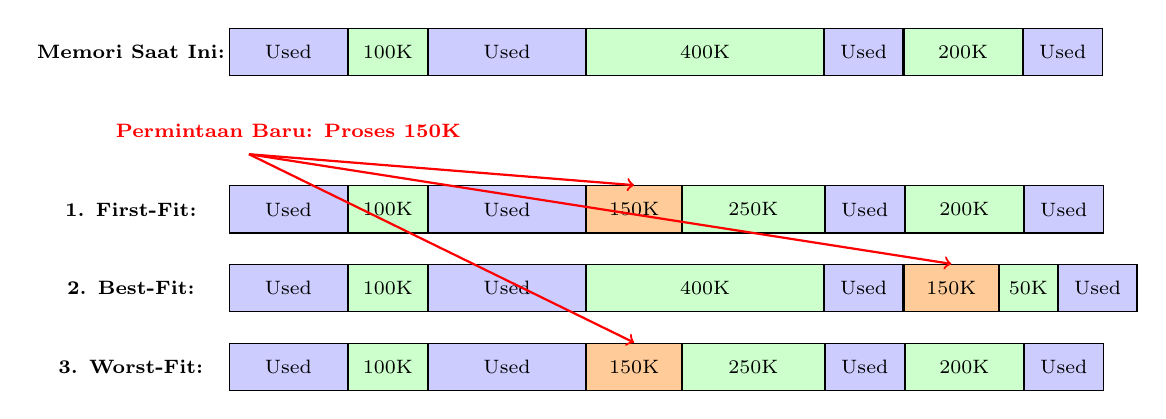
\begin{tikzpicture}[
        process/.style={draw, rectangle, minimum height=0.6cm, fill=blue!20, font=\scriptsize},
        hole/.style={draw, rectangle, minimum height=0.6cm, fill=green!20, font=\scriptsize},
        label/.style={font=\scriptsize\bfseries}
    ]
        % Base Memory State
        \node[label] at (-2, 2.5) {Memori Saat Ini:};
        
        \node[process, minimum width=1.5cm] (p1) at (0, 2.5) {Used};
        \node[hole, minimum width=1.0cm, right=0cm of p1] (h1) {100K};
        \node[process, minimum width=2.0cm, right=0cm of h1] (p2) {Used};
        \node[hole, minimum width=3.0cm, right=0cm of p2] (h2) {400K};
        \node[process, minimum width=1.0cm, right=0cm of h2] (p3) {Used};
        \node[hole, minimum width=1.5cm, right=0cm of p3] (h3) {200K};
        \node[process, minimum width=1.0cm, right=0cm of h3] (p4) {Used};

        % Request
        \node[label, text=red] at (0, 1.5) {Permintaan Baru: Proses 150K};

        % First-Fit
        \node[label] at (-2, 0.5) {1. First-Fit:};
        \node[process, minimum width=1.5cm] (f_p1) at (0, 0.5) {Used};
        \node[hole, minimum width=1.0cm, right=0cm of f_p1] (f_h1) {100K};
        \node[process, minimum width=2.0cm, right=0cm of f_h1] (f_p2) {Used};
        \node[process, minimum width=1.2cm, fill=orange!40, right=0cm of f_p2] (new1) {150K};
        \node[hole, minimum width=1.8cm, right=0cm of new1] (f_h2) {250K};
        \node[process, minimum width=1.0cm, right=0cm of f_h2] (f_p3) {Used};
        \node[hole, minimum width=1.5cm, right=0cm of f_p3] (f_h3) {200K};
        \node[process, minimum width=1.0cm, right=0cm of f_h3] (f_p4) {Used};
        \draw[->, thick, red] (-0.5, 1.2) -- (new1.north);

        % Best-Fit
        \node[label] at (-2, -0.5) {2. Best-Fit:};
        \node[process, minimum width=1.5cm] (b_p1) at (0, -0.5) {Used};
        \node[hole, minimum width=1.0cm, right=0cm of b_p1] (b_h1) {100K};
        \node[process, minimum width=2.0cm, right=0cm of b_h1] (b_p2) {Used};
        \node[hole, minimum width=3.0cm, right=0cm of b_p2] (b_h2) {400K};
        \node[process, minimum width=1.0cm, right=0cm of b_h2] (b_p3) {Used};
        \node[process, minimum width=1.2cm, fill=orange!40, right=0cm of b_p3] (new2) {150K};
        \node[hole, minimum width=0.3cm, right=0cm of new2] (b_h3) {50K};
        \node[process, minimum width=1.0cm, right=0cm of b_h3] (b_p4) {Used};
        \draw[->, thick, red] (-0.5, 1.2) -- (new2.north);

        % Worst-Fit
        \node[label] at (-2, -1.5) {3. Worst-Fit:};
        \node[process, minimum width=1.5cm] (w_p1) at (0, -1.5) {Used};
        \node[hole, minimum width=1.0cm, right=0cm of w_p1] (w_h1) {100K};
        \node[process, minimum width=2.0cm, right=0cm of w_h1] (w_p2) {Used};
        \node[process, minimum width=1.2cm, fill=orange!40, right=0cm of w_p2] (new3) {150K};
        \node[hole, minimum width=1.8cm, right=0cm of new3] (w_h2) {250K};
        \node[process, minimum width=1.0cm, right=0cm of w_h2] (w_p3) {Used};
        \node[hole, minimum width=1.5cm, right=0cm of w_p3] (w_h3) {200K};
        \node[process, minimum width=1.0cm, right=0cm of w_h3] (w_p4) {Used};
        \draw[->, thick, red] (-0.5, 1.2) -- (new3.north);

    \end{tikzpicture}
\end{frame}

\begin{frame}
    \frametitle{Contoh Soal Strategi Alokasi}
    \framesubtitle{Simulasi alokasi blok memori}
    \small
    \begin{block}{Soal}
        Diberikan sekumpulan blok memori kosong (\textit{free holes}) secara berurutan di RAM dengan ukuran: 
        \tem{100K}, \tem{500K}, \tem{200K}, \tem{300K}, dan \tem{600K}.
        
        Terdapat 4 proses baru yang datang dan masing-masing meminta alokasi secara berurutan:
        \tem{212K}, \tem{417K}, \tem{112K}, dan \tem{624K}.

        Tentukan partisi \textit{hole} mana yang akan diisi oleh proses-proses tersebut dengan algoritma:
        \begin{enumerate}
            \item \textbf{First-Fit}
            \item \textbf{Best-Fit}
            \item \textbf{Worst-Fit}
        \end{enumerate}
    \end{block}
\end{frame}

\begin{frame}
    \frametitle{Jawaban: First-Fit}
    \framesubtitle{Langkah-langkah simulasi}
    \small
    \textbf{Memori Awal:} [100K] [500K] [200K] [300K] [600K]
    
    \begin{enumerate}
        \item \textbf{Proses 212K:} First-Fit mencari blok pertama yang $\ge$ 212K.
        \begin{itemize}
            \item Masuk ke blok \textbf{500K}. Sisa blok: 500K - 212K = \textbf{288K}.
            \item \textit{Status:} [100K] \textcolor{blue}{[212K dipakai] [288K sisa]} [200K] [300K] [600K]
        \end{itemize}
        \item \textbf{Proses 417K:} Mencari blok pertama yang $\ge$ 417K.
        \begin{itemize}
            \item Masuk ke blok \textbf{600K}. Sisa blok: 600K - 417K = \textbf{183K}.
            \item \textit{Status:} [100K] [...] [288K sisa] [200K] [300K] \textcolor{blue}{[417K dipakai] [183K sisa]}
        \end{itemize}
        \item \textbf{Proses 112K:} Mencari blok pertama yang $\ge$ 112K.
        \begin{itemize}
            \item Masuk ke blok sisa \textbf{288K}. Sisa blok: 288K - 112K = \textbf{176K}.
        \end{itemize}
        \item \textbf{Proses 624K:} Mencari blok pertama yang $\ge$ 624K.
        \begin{itemize}
            \item Karena blok sisa tidak ada yang mencukupi, harus \tem{menunggu}.
        \end{itemize}
    \end{enumerate}
\end{frame}

\begin{frame}
    \frametitle{Jawaban: Best-Fit}
    \framesubtitle{Langkah-langkah simulasi}
    \small
    \textbf{Memori Awal:} [100K] [500K] [200K] [300K] [600K]
    
    \begin{enumerate}
        \item \textbf{Proses 212K:} Best-Fit mencari sisa blok terkecil yang $\ge$ 212K (yakni blok 300K).
        \begin{itemize}
            \item Masuk ke blok \textbf{300K}. Sisa blok: 300K - 212K = \textbf{88K}.
            \item \textit{Status:} [100K] [500K] [200K] \textcolor{blue}{[212K dipakai] [88K sisa]} [600K]
        \end{itemize}
        \item \textbf{Proses 417K:} Mencari sisa blok terkecil yang $\ge$ 417K.
        \begin{itemize}
            \item Masuk ke blok \textbf{500K}. Sisa blok: 500K - 417K = \textbf{83K}.
        \end{itemize}
        \item \textbf{Proses 112K:} Mencari sisa blok terkecil yang $\ge$ 112K.
        \begin{itemize}
            \item Masuk ke blok \textbf{200K}. Sisa blok: 200K - 112K = \textbf{88K}.
        \end{itemize}
        \item \textbf{Proses 624K:} Mencari sisa blok terkecil yang $\ge$ 624K.
        \begin{itemize}
            \item Karena blok sisa tidak ada yang mencukupi (terbesar tinggal 600K, sisa yang lain terlalu kecil), harus \tem{menunggu}.
        \end{itemize}
    \end{enumerate}
\end{frame}

\begin{frame}
    \frametitle{Jawaban: Worst-Fit}
    \framesubtitle{Langkah-langkah simulasi}
    \small
    \textbf{Memori Awal:} [100K] [500K] [200K] [300K] [600K]
    
    \begin{enumerate}
        \item \textbf{Proses 212K:} Worst-Fit mencari sisa blok terbesar yang $\ge$ 212K (yakni blok 600K).
        \begin{itemize}
            \item Masuk ke blok \textbf{600K}. Sisa blok: 600K - 212K = \textbf{388K}.
            \item \textit{Status:} [100K] [500K] [200K] [300K] \textcolor{blue}{[212K dipakai] [388K sisa]}
        \end{itemize}
        \item \textbf{Proses 417K:} Mencari sisa blok terbesar yang $\ge$ 417K.
        \begin{itemize}
            \item Masuk ke blok \textbf{500K}. Sisa blok: 500K - 417K = \textbf{83K}.
        \end{itemize}
        \item \textbf{Proses 112K:} Mencari sisa blok terbesar yang $\ge$ 112K.
        \begin{itemize}
            \item Masuk ke blok sisa \textbf{388K}. Sisa blok: 388K - 112K = \textbf{276K}.
        \end{itemize}
        \item \textbf{Proses 624K:} Mencari sisa blok terbesar yang $\ge$ 624K.
        \begin{itemize}
            \item Karena blok sisa tidak ada yang mencukupi, harus \tem{menunggu}.
        \end{itemize}
    \end{enumerate}
\end{frame}

\section{Fragmentasi Memori}

\begin{frame}
    \frametitle{Apa itu Fragmentasi Memori?}
    \framesubtitle{Konsekuensi tak terhindarkan dari dinamika OS}
    \small
    \begin{block}{Definisi}
        Fragmentasi adalah kondisi di mana memori total cukup besar, tetapi terpecah menjadi banyak potongan-potongan terpisah yang sulit dimanfaatkan secara efisien.
    \end{block}
    \vspace{0.2cm}
    \begin{itemize}
        \item Muncul sebagai efek samping mekanisme alokasi dan dealokasi memori berulang-ulang.
        \item Menyebabkan \tem{pemborosan} kapasitas.
        \item Mengurangi efisiensi penggunaan sumber daya sistem seiring berjalannya operasi OS.
    \end{itemize}
\end{frame}

\begin{frame}
    \frametitle{Fragmentasi Eksternal vs Internal}
    \framesubtitle{Mengenali dua jenis tipe pemborosan memori}
    \small
    \begin{columns}[T]
        \column{0.48\textwidth}
        \textbf{Fragmentasi Eksternal}
        \begin{itemize}
            \item Ada ruang memori bebas di \textbf{luar} blok per-proses (di antara proses-proses).
            \item Total \textit{hole} cukup untuk proses baru, namun \tem{tidak berurutan / tidak kontigu}.
        \end{itemize}
        \vspace{3mm}
        \centering
        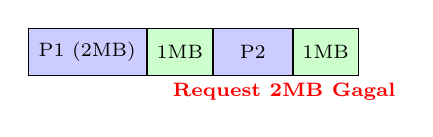
\begin{tikzpicture}
            \node[draw, rectangle, minimum height=0.6cm, minimum width=1.5cm, fill=blue!20, font=\scriptsize] (p1) {P1 (2MB)};
            \node[draw, rectangle, minimum height=0.6cm, minimum width=0.8cm, fill=green!20, font=\scriptsize, right=0cm of p1] (h1) {1MB};
            \node[draw, rectangle, minimum height=0.6cm, minimum width=1.0cm, fill=blue!20, font=\scriptsize, right=0cm of h1] (p2) {P2};
            \node[draw, rectangle, minimum height=0.6cm, minimum width=0.8cm, fill=green!20, font=\scriptsize, right=0cm of p2] (h2) {1MB};
            \node[font=\scriptsize\bfseries, text=red, yshift=-0.5cm] at (2.5,0) {Request 2MB Gagal};
        \end{tikzpicture}
        
        \column{0.48\textwidth}
        \textbf{Fragmentasi Internal}
        \begin{itemize}
            \item Ada ruang memori tak terpakai \textbf{di dalam} partisi proses itu sendiri.
            \item Terjadi bila unit memori yang dialokasikan ukurannya membulat kaku.
        \end{itemize}
        \vspace{3mm}
        \centering
        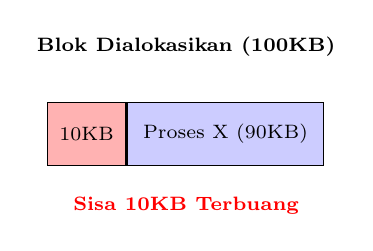
\begin{tikzpicture}
            \node[draw, rectangle, minimum height=0.8cm, minimum width=3.5cm, fill=gray!20] (block) {};
            \node[draw, rectangle, minimum height=0.8cm, minimum width=2.5cm, fill=blue!20, font=\scriptsize, left=0cm of block.east, anchor=east] (p) {Proses X (90KB)};
            \node[draw, rectangle, minimum height=0.8cm, minimum width=1.0cm, fill=red!30, font=\scriptsize, right=0cm of p.west, anchor=east] (h) {10KB};
            \node[font=\scriptsize\bfseries, yshift=0.7cm] at (block.north) {Blok Dialokasikan (100KB)};
            \node[font=\scriptsize\bfseries, text=red, yshift=-0.5cm] at (block.south) {Sisa 10KB Terbuang};
        \end{tikzpicture}
    \end{columns}
\end{frame}

\begin{frame}
    \frametitle{Fenomena 50 Percent Rule dan Kompaksi}
    \framesubtitle{Karakteristik Fragmentasi dan Solusinya}
    \small
    \begin{itemize}
        \item \textbf{50 Percent Rule}: Secara statistik, untuk strategi alokasi first-fit yang berjalan terus menerus secara acak, diperkirakan \tem{$1/3$ (sepertiga)} blok memori akan terbuang karena fragmentasi eksternal.
    \end{itemize}
    
    \begin{alertblock}{Solusi Konvensional: Kompaksi}
        Mengeser seluruh unit proses yang ada, memadatkannya jadi satu, sehingga semua sisa bebas (holes) memori dapat menyatu besar.
        \begin{itemize}
            \item \textbf{Kerugiannya:} Sangat mahal dalam hal \tem{overhead komputasi}. Semua pointer referensi dari sistem memory OS harus dirubah dan dihentikan seketika.
        \end{itemize}
    \end{alertblock}
\end{frame}

\section{Teori Paging}

\begin{frame}
    \frametitle{Apa Itu Paging?}
    \framesubtitle{Solusi Modern untuk RAM Tidak Bersambung}
    \small
    \begin{block}{Definisi Paging}
        Teknik manajemen memori yang memungkinkan alamat fisik memori dari suatu proses bisa dialokasikan \tem{secara noncontiguous} (tidak berurutan). Teknik Paging menyingkirkan masalah \textbf{Fragmentasi Eksternal} sepenuhnya.
    \end{block}
    
    \begin{itemize}
        \item \textbf{Memori Fisik} $\rightarrow$ Dipotong-potong ukurannya identik (blok tetap) yang dinamakan \textbf{Frame} (misal: 4KB).
        \item \textbf{Memori Logis / Virtual} $\rightarrow$ Dipotong-potong ukuran yang \textit{sama persis dengan Frame} dinamakan \textbf{Page}.
        \item \textbf{Keuntungan} $\rightarrow$ Tiap \textit{Page} unik dari sebuah program bebas diselipkan ke sembarang \textit{Frame} kosong manapun di RAM fisik. 
    \end{itemize}
\end{frame}

\begin{frame}
    \frametitle{Mapping antara Page dan Frame}
    \framesubtitle{Peran Page Table}
    \small
    \begin{columns}[T]
        \column{0.48\textwidth}
        \textbf{Page Table}
        \begin{itemize}
            \item Struktur tabel sentral di OS yang dialokasikan per proses sistem.
            \item Berfungsi \textbf{memetakan} info translasi dari mana \tem{Page Number} ke \tem{Frame Number} yang ada.
            \item Unit \textbf{MMU} (Memory Management Unit) menggunakan tabel ini setiap milidetik secara hardware.
        \end{itemize}
        \column{0.48\textwidth}
        \begin{alertblock}{Konsep Kunci}
            Ukuran \textit{Page} dan ukuran \textit{Frame} \textbf{harus persis sama} untuk memastikan proses pemetaan (mapping) berjalan dengan valid dan efisien!
        \end{alertblock}
    \end{columns}
\end{frame}

\begin{frame}
    \frametitle{Keunggulan Arsitektur Paging}
    \framesubtitle{Konsep Teoritis Paging}
    \small
    \begin{columns}[T]
        \column{0.48\textwidth}
        \textbf{Memori Logis (Proses)}
        \begin{itemize}
            \item Ruang alamat pengguna/proses dibagi ke \textit{page} ukuran statis.
            \item Program menganggap memorinya linear dan bersambung.
        \end{itemize}
        \vspace{3mm}
        \textbf{Memori Fisik (RAM)}
        \begin{itemize}
            \item Dibagi ke \textit{frame} ukuran statis.
            \item Dialokasikan secara acak noncontiguous sesuai ketersediaan.
        \end{itemize}
        \column{0.48\textwidth}
        \begin{alertblock}{Mengapa Paging Sangat Baik?}
            \begin{itemize}
                \item Benar-benar mengatasi \textbf{Fragmentasi Eksternal}.
                \item Menyederhanakan alokasi: OS bebas menempatkan \textit{page} tanpa mencari blok berurutan.
                \item Terisolasi dengan baik, dan dapat mendukung penggunaan share memory.
            \end{itemize}
        \end{alertblock}
    \end{columns}
\end{frame}

\section{Ringkasan dan Latihan}

\begin{frame}
    \frametitle{Ringkasan Super Singkat (6 Kalimat Kunci)}
    \framesubtitle{Jika lupa materi, ingat 6 poin ini}
    \small
    \begin{enumerate}
        \item Alokasi memori berurusan dengan metode OS meletakkan blok memori target proses ke celah kosong ruang memori (\textit{hole}).
        \item Algoritma \textit{First-fit} paling cepat, sedang \textit{Best-fit} terbaik efisiensinya tapi menumpukkan ruang \textit{fragmented holes}.
        \item Pemborosan sisa partisi luasan blok tidak kontigu dinamakan sebagai \tem{Fragmentasi Eksternal}.
        \item Konsep teoritis memori modern dengan nama \textbf{Paging} digunakan khusus mengelola data proses terpencar (\tem{noncontiguous}).
        \item Proses Virtual dieksekusi bernama \textit{Page}, Kapling Fisikal penampung dinamakan \textit{Frame}.
        \item Entitas \textit{Page Table} senantiasa dilirik oleh MMU hardware sebagai rujukan menerjemahkan Alamat Maya menuju Alamat RAM Sejati.
    \end{enumerate}
\end{frame}

\begin{frame}
    \frametitle{Latihan Mandiri}
    \framesubtitle{Kerjakan pelan, diskusikan berpasangan}
    \small
    \begin{enumerate}
        \item Diberitahukan ada sisa luang ruang memori RAM berurutan (\textit{holes}) masing-masing: \textbf{15K, 30K, 40K, 25K}. \\
        Terdapat sebuah Proses C berukuran \textbf{22K}. Apakah perbandingan blok partisi tujuan dialokasikan OS apabila OS menerapkan metode strategi implementasi berikut?
        \begin{itemize}
            \item First-Fit?
            \item Best-Fit?
            \item Worst-Fit?
        \end{itemize}
        \item Mengapa defragmentasi memori (Kompaksi) secara rutin dalam OS modern amat jarang dijalankan / tidak efisien?
    \end{enumerate}
\end{frame}

\begin{frame}
    \frametitle{Jawaban Latihan Mandiri}
    \framesubtitle{Solusi latihan alokasi kustom}
    \small
    \begin{enumerate}
        \item \textbf{Jawaban Alokasi (Kondisi Awal: 15K, 30K, 40K, 25K):}
        \begin{itemize}
            \item \textbf{First-Fit:} Proses 22K akan menempati \textbf{blok 30K} karena ini adalah *hole* pertama yang mencukupi untuk 22K (yang 15K dilewati karena kekecilan).
            \item \textbf{Best-Fit:} Proses 22K akan mencari sisa terkecil, jadi akan masuk ke \textbf{blok 25K}. Sisa blok 3K.
            \item \textbf{Worst-Fit:} Proses 22K mencari *hole* terbesar, jadi akan menempati \textbf{blok 40K}. Sisa blok 18K.
        \end{itemize}
        \vspace{0.4cm}
        \item \textbf{Jawaban Kompaksi:} Kompaksi sangat dihindari karena berfokus untuk menyatukan ruang dengan menggeser proses-proses di memori secara fisik. Hal ini menyebabkan \tem{overhead komputasi} yang tinggi karena CPU dan MMU harus mendata ulang register maupun cache dari seluruh relokasi alamat memori yang berpindah.
    \end{enumerate}
\end{frame}

\begin{frame}
    \frametitle{Terima Kasih}
    \begin{center}
        \Huge \textbf{Ada Pertanyaan?}

        \vspace{0.8cm}
        \normalsize
        Persiapkan mental di materi Week ke-7 untuk masuk lebih detail tentang lanjutan mekanisme \tem{Virtual Memory} Modern dan Swapping.
    \end{center}
\end{frame}

\end{document}
